%label:"fig:VanishingPathsForP2"
%type:"figure"
%name:"vanishing paths for P2"
%caption:"A set of vanishing paths for the Lefschetz fibration $W(z_1, z_2) = z_1 + z_2 + (z_1z_2)^{-1}$"
%parent:"exm_MirrorSymmetryForP2"


    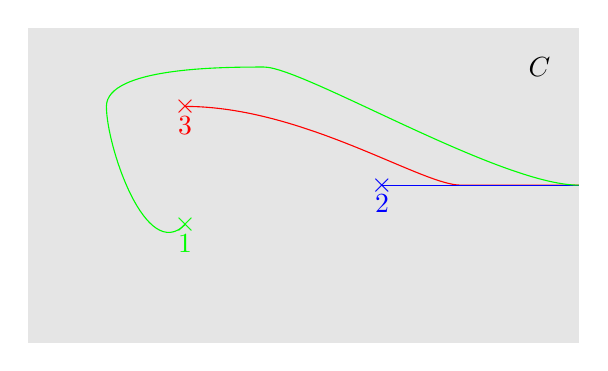
\begin{tikzpicture}

        \fill[gray!20] (-3,2.5) rectangle (4,-1.5);
        
        \node at (3.5,2) {$\mathbb{C}$};
        
        \node[green] at (-1,0) {$\times$};
        \node[blue] at (1.5,0.5) {$\times$};
        \node[red] at (-1,1.5) {$\times$};
        
        \node[below,green] at (-1,0) {$1$};
        \node[below,blue] at (1.5,0.5) {$2$};
        \node[below,red] at (-1,1.5) {$3$};
        \draw[red] (-1,1.5) .. controls (0.5,1.5) and (2,0.5) .. (2.5,0.5) .. controls (3,0.5) and (3.5,0.5) .. (4,0.5);
        \draw[blue] (1.5,0.5) -- (4,0.5);
        \draw[green] (-1,0) .. controls (-1.5,-0.5) and (-2,1) .. (-2,1.5) .. controls (-2,2) and (-0.5,2) .. (0,2) .. controls (0.5,2) and (3,0.5) .. (4,0.5);
    \end{tikzpicture}

